
\begin{frame}
\frametitle{Representations of Boolean functions}

\begin{center}
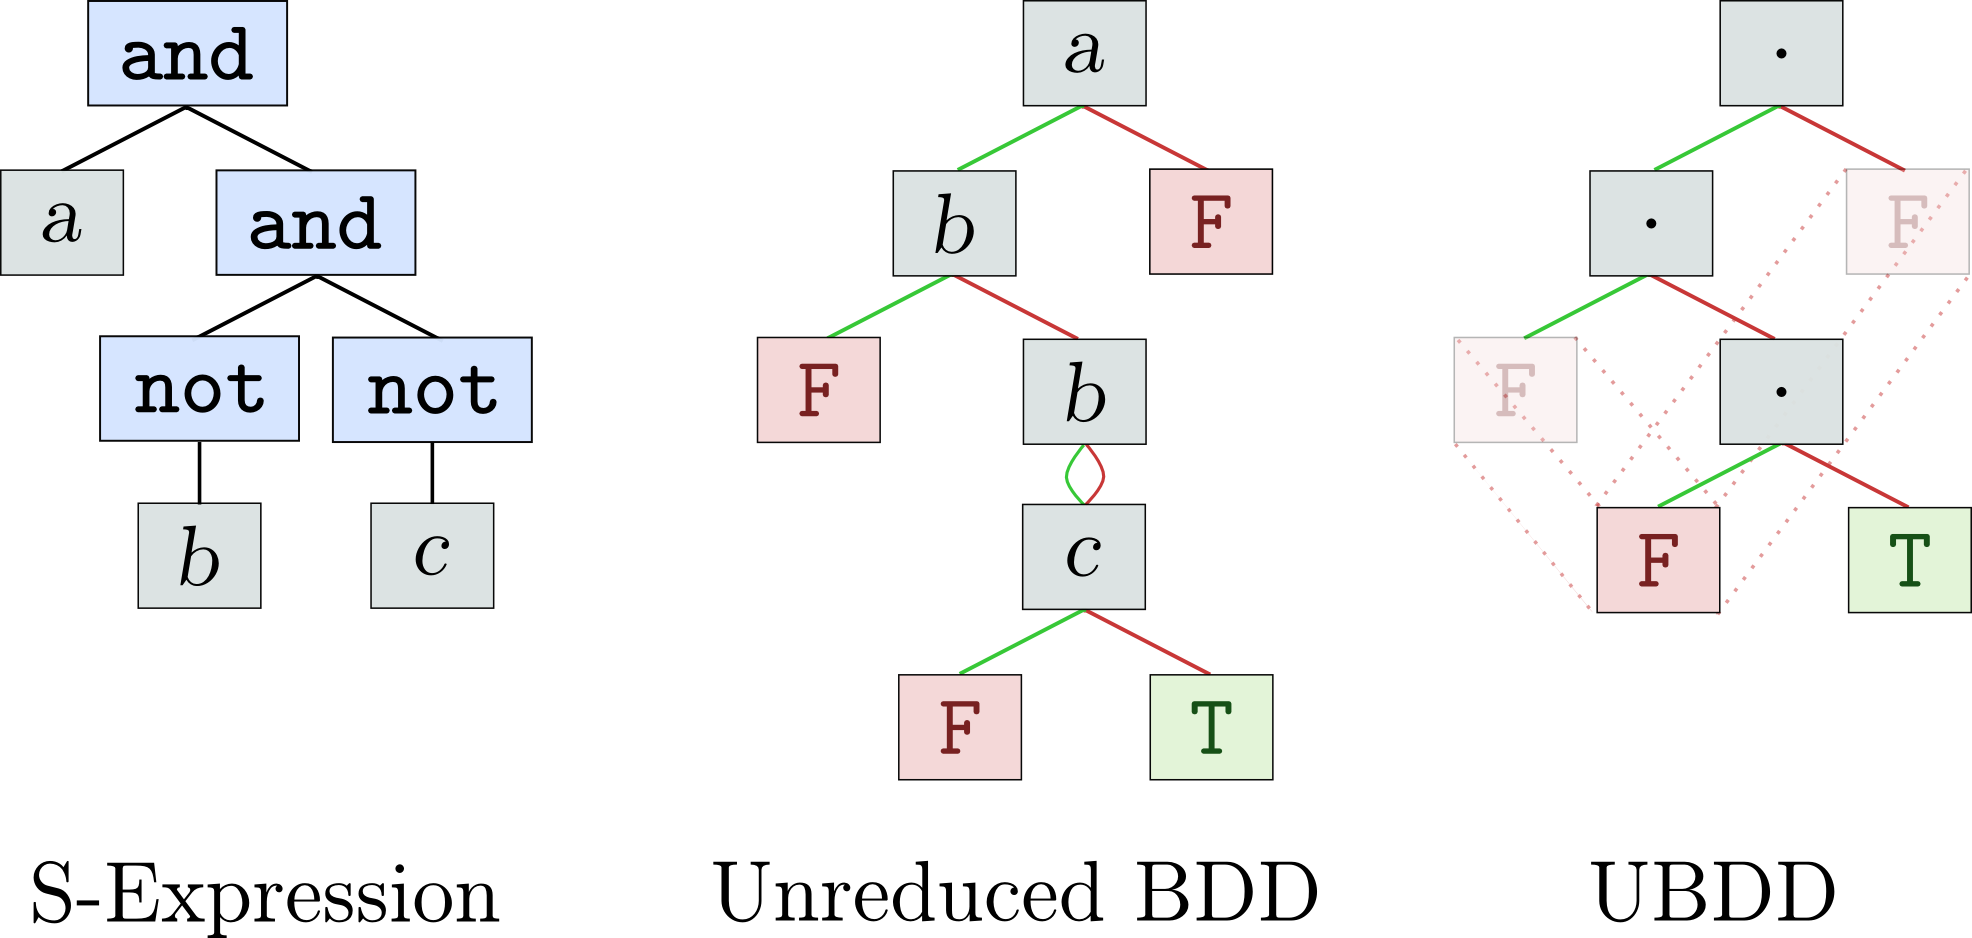
\includegraphics[width=11cm]{reps.png}
\end{center}

\end{frame}



\begin{frame}
\frametitle{Interpreting representations of Boolean functions}

In most representations, meanings are given by \Highlight{environments} mapping
variables to values

\begin{itemize}
\item \Code{(eval T env) = T}
\item \Code{(eval NIL env) = NIL}
\item \Code{(eval var env) = (lookup var env)}
\item \Code{(eval `(and ,a ,b) env) = (and (eval a env) (eval b env))}
\item \Code{(eval `(or ,a ,b) env) = (or (eval a env) (eval b env))}
\item \Code{(eval `(not ,a) env) = (not (eval a env))}
\end{itemize}

%% \SmallSkip
%% Example: if $f$ is \Code{(and a (and (not b) (not c)))}, then:
%% \begin{itemize}
%% \item \Code{(eval $f$ \{a $\leftarrow$ T, b $\leftarrow$ NIL, c $\leftarrow$ T\}) = NIL}
%% \item \Code{(eval $f$ \{a $\leftarrow$ T, b $\leftarrow$ NIL, c $\leftarrow$ NIL\}) = T}
%% \end{itemize}

\end{frame}



\begin{frame}
\frametitle{Interpreting UBDDs}

For UBDDs, meanings are given by \Highlight{list of values} telling us to go left
or right as we descend

\begin{itemize}
\item \Code{(eval-ubdd T vals) = T}
\item \Code{(eval-ubdd NIL vals) = NIL}
\item \Code{(eval-ubdd `(,a $.$ ,b) T::vals) = (eval-ubdd a vals)}
\item \Code{(eval-ubdd `(,a $.$ ,b) NIL::vals) = (eval-ubdd b vals)}
\end{itemize}

%% \SmallSkip

%% Let $f$ be \Code{(\Highlight{(NIL $.$ (NIL $.$ T))} $.$ NIL)}
%% \begin{itemize}
%% \item \Code{(eval-bdd $f$ [T, NIL, T]) = NIL}
%% \item \Code{(eval-bdd $f$ [T, NIL, NIL]) = T}
%% \end{itemize}

\end{frame}


%% \begin{frame}[fragile]
%% \frametitle{UBDDs Can Represent all Boolean Functions}

%% \begin{verbatim}
%% (defthm normp-of-q-ite
%%   (implies (and (normp a)
%%                 (normp b)
%%                 (normp c))
%%            (normp (q-ite a b c))))

%% (defthm eval-bdd-of-q-ite
%%   (equal (eval-bdd (q-ite a b c) vals)
%%          (if (eval-bdd a vals)
%%              (eval-bdd b vals)
%%            (eval-bdd c vals))))
%% \end{verbatim}
%% \end{frame}

\begin{frame}
\frametitle{Canonicity}

For UBDDs, the following statements are equivalent
\begin{itemize}
\item x = y
\item $\forall$ vals : \Code{(eval-ubdd x vals)} $=$ \Code{(eval-ubdd y vals)}
\end{itemize}

\SmallSkip
Many Boolean-function representations do not have this property
\begin{itemize}
\item \Code{(not a)} vs. \Code{(not (not (not a)))}
\end{itemize}

\SmallSkip

Efficiency characteristics
\begin{itemize}
\item Expensive to construct
\item Cheap to compare (pointer equality)
\end{itemize}

\end{frame}



\begin{frame}[fragile]
\begin{verbatim}
(defun normp (x)
  (if (atom x)
      (booleanp x)
    (and (normp (car x))
         (normp (cdr x))
         (if (atom (car x))
             (not (equal (car x) (cdr x)))
           t))))

(defun q-not (x)
  (if (atom x)
      (if x nil t)
    (hons (q-not (car x))
          (q-not (cdr x)))))
\end{verbatim}
\end{frame}


\begin{frame}[fragile]
\begin{verbatim}
(defun q-ite (x y z)
  (cond ((null x) z)
        ((atom x) y)
        (t 
         (let ((y (if (hons-equal x y) t y))
               (z (if (hons-equal x z) nil z)))
           (cond ((hons-equal y z)
                  y)
                 ((and (eq y t) (eq z nil))
                  x)
                 ((and (eq y nil) (eq z t))
                  (q-not x))
                 (t 
                  (qcons 
                   (q-ite (car x) (qcar y) (qcar z))
                   (q-ite (cdr x) (qcdr y) (qcdr z)))))))))
\end{verbatim}
\end{frame}


\begin{frame}[fragile]
\begin{verbatim}
(defun q-and (x y)
  (cond ((atom x)
         (if x 
             (if (atom y) 
                 (if y t nil) 
               y)
           nil))
        ((atom y)
         (if y x nil))
        ((hons-equal x y)
         x)
        (t
         (qcons (q-and (car x) (car y))
                (q-and (cdr x) (cdr y))))))
\end{verbatim}
\end{frame}

